\documentclass[conference]{IEEEtran}
\IEEEoverridecommandlockouts
% The preceding line is only needed to identify funding in the first footnote. If that is unneeded, please comment it out.
\usepackage{cite}
\usepackage{amsmath,amssymb,amsfonts}
\usepackage{algorithmic}
\usepackage{graphicx}
\usepackage{hyperref}
\usepackage{subcaption}
\usepackage{textcomp}
\usepackage{xcolor}
\def\BibTeX{{\rm B\kern-.05em{\sc i\kern-.025em b}\kern-.08em
    T\kern-.1667em\lower.7ex\hbox{E}\kern-.125emX}}

\hypersetup{
    colorlinks=true,
    linkcolor=blue,
    filecolor=magenta,
    urlcolor=cyan,
}

\begin{document}

\title{FaceNet Clustering Analysis}

\author{
\IEEEauthorblockN{Rodrigo Castiel}
\IEEEauthorblockA{\textit{Center for Informatics} \\
\textit{Federal University of Pernambuco}\\
Recife, Brazil \\
rcrs2@cin.ufpe.br}
}


\maketitle

\begin{abstract}
In the last decade, deep-learning based techniques brought us a remarkable breakthrough in face recognition.
Recently, Google Researchers proposed \textit{FaceNet}, a novel face recognition system that learns a mapping from face pictures to a feature-space where similarities are well described by simple euclidean distances \cite{??}.
FaceNet may be combined with different clustering methods and classifiers; on famous face recognition databases, it currently achieves the best accuracy.
In this paper, we use FaceNet as a feature extractor to perform a clustering analysis on three different databases: a small personal dataset, Labeled Faces in the Wild (LFW) and MUCT.
We run k-means, agglomerative clustering, spectral clustering, DBSCAN and mean-shift with different parameters on all datasets.
Experiments show that both DBSCAN and mean-shift achieve the best adjusted rand scores without even knowing the number of clusters in advance.

\end{abstract}

\begin{IEEEkeywords}
clustering, deep-learning, face recognition, facenet
\end{IEEEkeywords}

\section{Introduction}

\section{Related Work}

\section{Clustering Analysis}

\subsection{Databases}

Describe the purpose of each database.

Describe each database - number of points, clusters, and filters.

\begin{figure}[h]
\label{tsne_view_personal_faces}
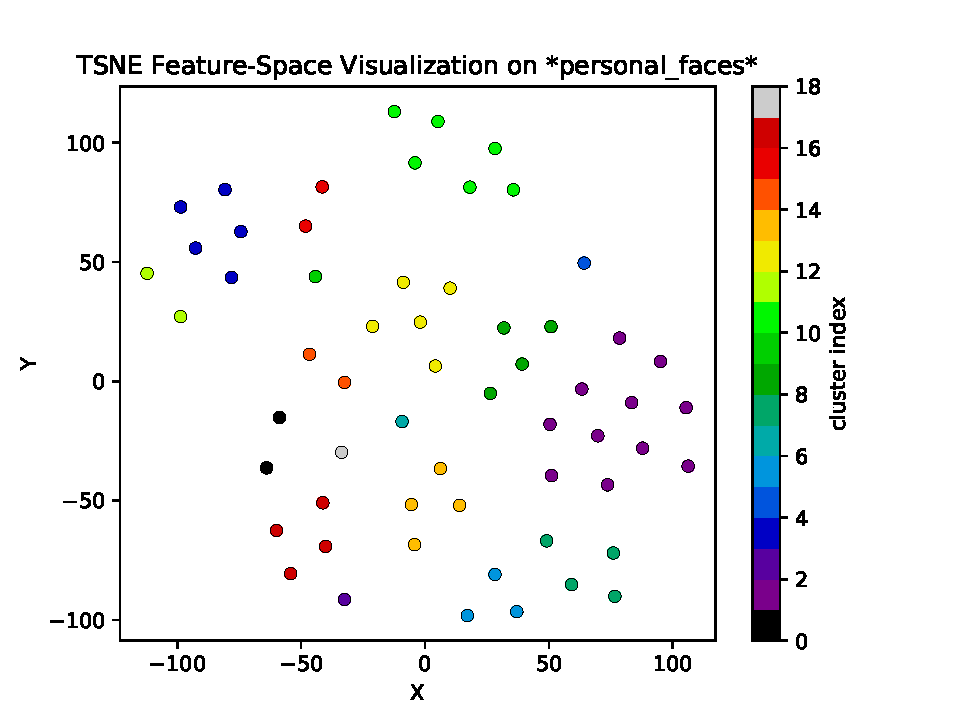
\includegraphics[width=\linewidth]{tsne_view_personal_faces}
\caption{TSNE visualization in feature-space on personal\_faces database.}
\end{figure}

\begin{figure}[h]
\label{tsne_view_lfw}
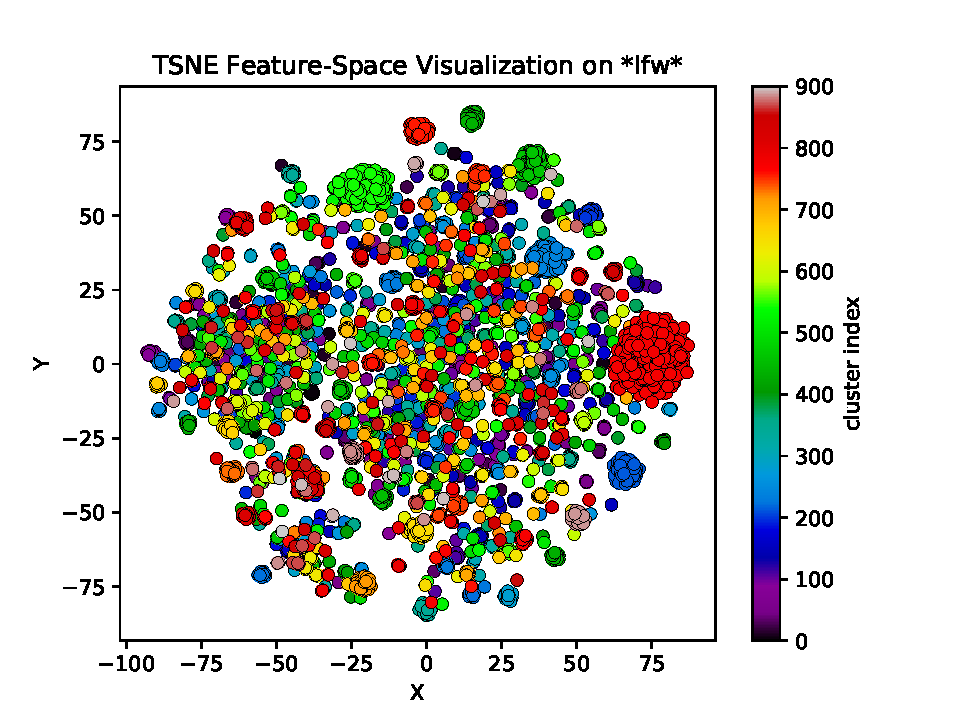
\includegraphics[width=\linewidth]{tsne_view_lfw}
\caption{TSNE visualization in feature-space on LFW database.}
\end{figure}

\begin{figure}[h]
\label{tsne_view_muct}
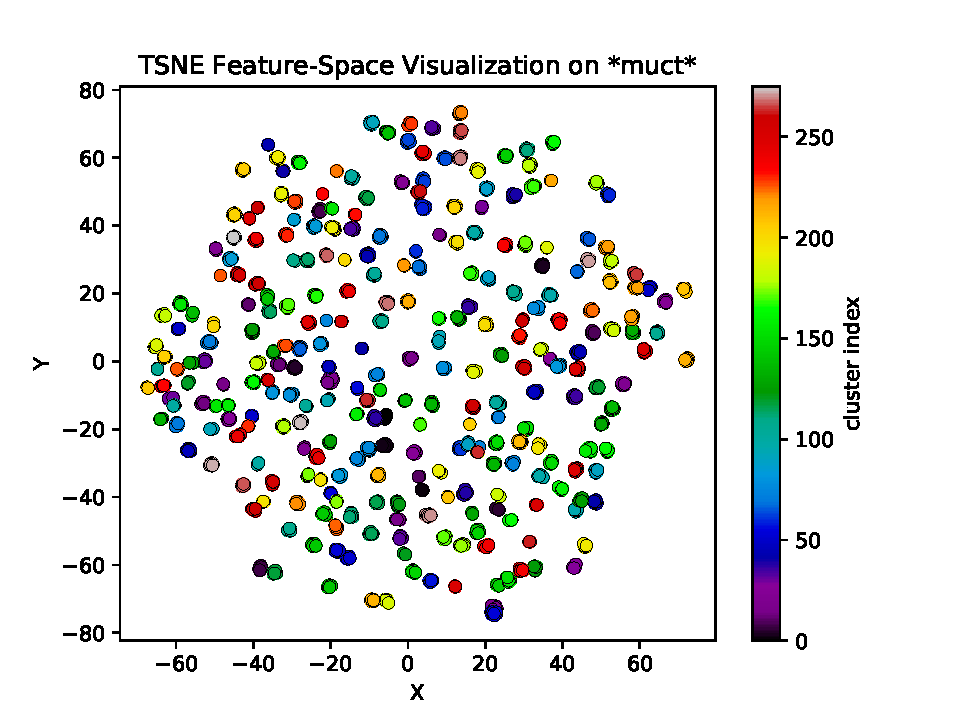
\includegraphics[width=\linewidth]{tsne_view_muct}
\caption{TSNE visualization in feature-space on MUCT database.}
\end{figure}

\subsection{Experiments}

Add picture of the experiments pipeline.

Explain how each clustering method was validated (fraction of dataset and number of times).

Explain two groups of methods: K-based (how K is automatically computed) and the other two.

Define metrics (adjusted rand score).

\subsection{Results}

\subsubsection{Score Analysis}

Add table of all average scores (method vs. dataset).

Briefly explain table results.

Explain why DBSCAN and mean-shift are the best options.

\subsubsection{DBSCAN and Mean-shift parameter analysis}

Add plot of score vs eps and score vs bandwidth.

Explain plots.

\subsubsection{Semantics Analysis}

Explain secondary tool that groups photos.

Write about problems with sunglasses, ethnical groups, etc.

Write that agglomerative clustering finds the best grouping when K is known.

\section{Conclusion}

Write about the advantages of DBSCAN and mean-shift.

Write about downsides of facenet (sunglasses, for example).
Explain why classification can be better than clustering.

\begin{thebibliography}{00}
\bibitem{b1} Francisco de A.T. de Carvalho, Eduardo C. Simões, Lucas V.C. Santana, Marcelo R.P. Ferreira,
Gaussian kernel c-means hard clustering algorithms with automated computation of the width hyper-parameters,
Pattern Recognition,
Volume 79,
2018,
Pages 370-386,
ISSN 0031-3203,
https://doi.org/10.1016/j.patcog.2018.02.018.

\bibitem{b2} Vision Group, University of Massachusetts, 
Image Segmentation Data,
http://archive.ics.uci.edu/ml/machine-learning-databases/image/.

\end{thebibliography}

\end{document}
